\documentclass{article}
\usepackage[margin=1in]{geometry}
\usepackage{graphicx}
\usepackage{multicol}
% \usepackage{multirow}
\usepackage{cite}

\title{Project 2\\Using a Feed-Forward Neural Network with a Sigmoid Activation Function and Supervised Learning Techniques to Approximate Parametric Curves}

\author{Christian Mann and Steven Reed \\
		University of Tulsa}

\begin{document}

\maketitle

\begin{multicols}{2}

\begin{abstract}
In this paper we develop our own Feed-Forward neural network based off of previous examples found in the book, Fundamentals of Computational neuroscience \cite{trappenberg}, and on the Internet. Our neural network features backpropagation for supervised learning. We then use it to approximate two parametric functions.
\end{abstract}

\section{Introduction}

A neural network can take many forms, but the ideas behind them all are derived from studies in the field of neuroscience. The general concept behind the structure of a neural network is simple to understand. A graph structure is created with a set of weighted edges. Some nodes are designated as inputs, some designated as outputs, and the rest are used for computation and are called ``hidden nodes''. By using an activation function to determine how inputs propagate, the network calculates a set of outputs.

As simple as this concept is, it proves to be an incredibly difficult challenge to create a network of any use. The purpose of a neural network is, in short, to approximate a function. Sometimes this function is known explicitly, but is difficult or expensive to compute. Other times the function cannot be explicitly known, but we can gather empirical data relating to the function and use it to create a network. Ultimately, the goal of a neural network is to approximate a function using whatever information about the function that we can get our hands on.

There are two main techniques in developing the structure of a neural network. The first technique is called Supervised Learning where the network is ``trained'' by means of giving it example inputs and outputs from the function we want it to approximate. After pouring over the examples over and over, the network (hopefully) converges to a certain structure and becomes well equipped at mimicking the original function. It does this by making many small changes to the weights associated with the edges in the network using a method known as ``backpropagation'' \cite{trappenberg}. The second popular method for constructing a neural network is known as Unsupervised Learning where the desired outcome is not known and the machine is responsible for finding correlations. We do not use any Unsupervised Learning techniques in this project.

In this project we wrote our own neural network in C++. We then used it to approximate various functions. These functions included the XOR function, a parametric circle, and complex parametric curve illustrating a coffee cup.

\section{Building a neural network}

We began by researching existing neural networks to get an idea for what kind of elements should be present in a network. There are many already availabe, and all have a varying set of features and capabilities. Many implementations are able to take advantage of a computer's GPU to parallelize the computations. The most simplistic example network we could find, though, was a Javascript implementation known as Brain.js \cite{brain}. We used Brain.js as a guide for creating our own neural network in C++ with the hopes of performing faster than Javascript at a lower level, but still without any hope to achieve the performance of a GPGPU solution.

We chose to use a Sigmoid activation function, $S(t)$, for its simplicity and convenient derivative. The convenient derivative is important as it will be computed a lot during training. Using a non-linear activation function also keeps our network from being limited to approximating linear functions \cite{hornik}. The derivative is used to modify error terms for each node which are eventually used to effect the change in weight to incoming edges. Since the derivate of the sigmoid function is highest for values around 0 ($S(0) = 0.5$ is a global maxima), multiplying the error by the derivative tends to favor errors associated with outputs where $S(output)\approx0.5$, in turn causing them to adjust weights quicker.

	\[S(t) = \frac{1}{1+e^{-t}}\]
	\[\frac{d}{dt}S(t) = S(t) * (1-S(t))\]

In addition to the use of the Sigmoid function for node activation, we discovered the use of a momentum factor in Brain.js which we also incorporated in our own model. The momentum is intended to help the network avoid local minima by increasing any change made to a given edge during training by some fraction of the change made to the edge on the previous iteration. It is intuitive to think of this as momentum; after an edge has a large change applied to it, the edge will continue to be changed by successively smaller amounts for several iterations afterward, even if there is no error detected in the node. While this at first sounds like unwanted behavior, the intention is to try and avoid local minima in approximation of the function.

The primary initial parameters that must be set prior to running our network are learning rate, momentum, hidden layer dimensions, error threshold, and maximum iterations. The learning rate constant can be thought of as a magnitude adjustment on every change that occurs to an edge during training. The momentum constant determines how much change is retained and reapplied to the next change. The hidden layer dimensions determine how many hidden layers there are and how many nodes are in each layer. The layers are not required to contain the same number of nodes. Lastly the error threshold and the maximum iterations constants are used as stopping conditions. Once either threshold has been met, the network will consider the training finished. At this point, the network can be used just like the original function.

\section{Approximating the XOR Function}

Once the network was approaching completion, the first function we used to begin testing the network was the simple, yet popular, XOR function. After some debugging and fine tuning, we were able to build a network of 5 nodes (2 input, 1 output, and 1 hidden layer with 2 nodes) which was trained to approximate XOR. The only training patterns given were the 4 boolean expressions in Table~\ref{tab:xortable}, but each one was used to train the network roughly 4000 times to achieve adequate results with a sufficiently low error. The results of the inputs being fed through the resulting trained network can be seen in the right hand column of Table~\ref{tab:xortable}.

However, we were not satisfied to know that XOR performed appropriately for exactly the inputs we fed it repeatedly, we were curious what the rest of the output looked like after training. For example, what did $(I_1=0.34, I_2=0.64)$ look like? To see what the rest of the graph looked like, we fed the trained network a circle of $X$ and $Y$ inputs. We were surprised to see the gradual rise and fall of the 3D surface shown in Figure~\ref{fig:xor1} and Figure~\ref{fig:xor2}.

\section{Approximating a Parametric Circle}

Once we had the XOR function working properly, we wanted to step up the difficulty. In order to do this, we tried approximating a parametric function with one input as the $t$ value and two outputs for the $x$ and $y$ values. We created roughly 30 data points approximating the parametric plot of a circle, and trained the network for many iterations longer than the XOR function. We then used a validation set of 100 data-points of the same parametric plot to see how the network performed. The result can be seen in Figure~\ref{fig:circle} where the red circle is the actual validation set, and the blue circle is the one approximated by the network.

\section{Approximating a Parametric Coffee Cup}

As a more difficult challenge in parametric plot approximations, we used Wolfram Alpha to generate a parametric plot drawing of a coffee cup \cite{wolfram}. The equations used can be seen in Figure~\ref{fig:coffee-eqns}. The training data of the original plot can be seen in Figure~\ref{fig:coffee1} and consists of 300 points. Various starting parameters were used to try to approximate this coffee cup, but in the end it proved far too complex to do in a small amount of time on our limited hardware. After training the neural network for about 3 Million iterations, the graph in Figure~\ref{fig:coffee4} was achieved. The red outline is the training data while the blue outline is the output of the neural network. It's clear that the training had some significant effect, but did not converge as well as we had hoped. Some shapes are clearly defined, such as the outline of the steam on the right. Other sections, such as the handle and the body, make it clear what the network was going for, but still look like the drawing of a 3 year old. However, the right hand side of the saucer plate is a complete mess.

%\section{Weather Prediction}

%We wanted to use our network to learn something useful. We decided to attempt to use our network to predict the weather for Tulsa, Oklahoma. Because NOAA provides complete records for Tulsa from January of 1983\cite{noaa}, we had a large corpus of data: Each day has a min/max temperature, rainfall, wind velocity, and other such properties associated with it. We wrote a web scraper to extract the formatted data into a neutral format, so that we could work with it. After throwing out the days with bad data, we ended up with approximately 2300 data points. In order to make this fit our neural network, we decided to create datapoints of the form $f(day_{n}) = day_{n+1}$. Since there are $12$ properties per day, this means our network has $12$ inputs and $12$ outputs. We used three hidden layers of $5$ nodes each to approximate the function.

%Due to the large amount of data, we did not need to perform as many iterations through the data as other, smaller examples. In fact, after the first few hundred iterations, the neural network was essentially fully trained, with the error on the validation set fairly low. Some sample predictions are shown in Table~\ref{tab:weather}. Unfortunately, the network did not appear to learn anything useful about the weather in Oklahoma. It only appears to have learned averages for climate data, as can be seen from the output.

\section{Conclusion and Future Work}

It is clear that our network approximates functions to some extent, however, it is also clear that it could benefit from more features. Trying other non-linear activation functions than our chosen Sigmoid would be one way to generate different, and perhaps more accurate, networks. Another way would be to try various parameter settings for learning rate, momentum, hidden layer dimensions, and training/validation sets. We have found that finding the right parameter settings can be just as hard of a problem as finding the right network weights. If we really wanted to speed things up, we could try to parallelize the computations on a GPU. However, this is outside the scope of our current expertise.

At the start of the project, we wanted to use the network, along with some weather data, to try and approximate a weather forecast for Tulsa, OK. In the time allotted for the project, we were able to run some tests, but ultimately we were not able to gather data of any use. Due to the complexity of the problem, to really create good tests we would need to try several different initial parameters and run them each for long periods of time. The time and cost required to do this would easily be more than we have this semester. However, it is likely that such tests would be better suited for a more featured parallel neural network rather than our toy network built for this project.

\bibliographystyle{abbrv}
\bibliography{citations}

\end{multicols}

\pagebreak

\begin{table}[ht]
	\caption{XOR Truth Table}
	\label{tab:xortable}
	\begin{center}
		\begin{tabular}{cc|cc}
		\hline
		\hline
		\textbf{$In_1$} & \textbf{$In_2$} & \textbf{$Out$} & neuralnet \\
		\hline
			$0.0$ & $0.0$ & $0.0$ & $0.0062$\\
			$0.0$ & $1.0$ & $1.0$ & $0.9934$\\
			$1.0$ & $0.0$ & $1.0$ & $0.9934$\\
			$1.0$ & $1.0$ & $0.0$ & $0.0086$\\
		\hline

		\hline
		\end{tabular}
	\end{center}
\end{table}


\begin{figure}[tb]
	\begin{center}
		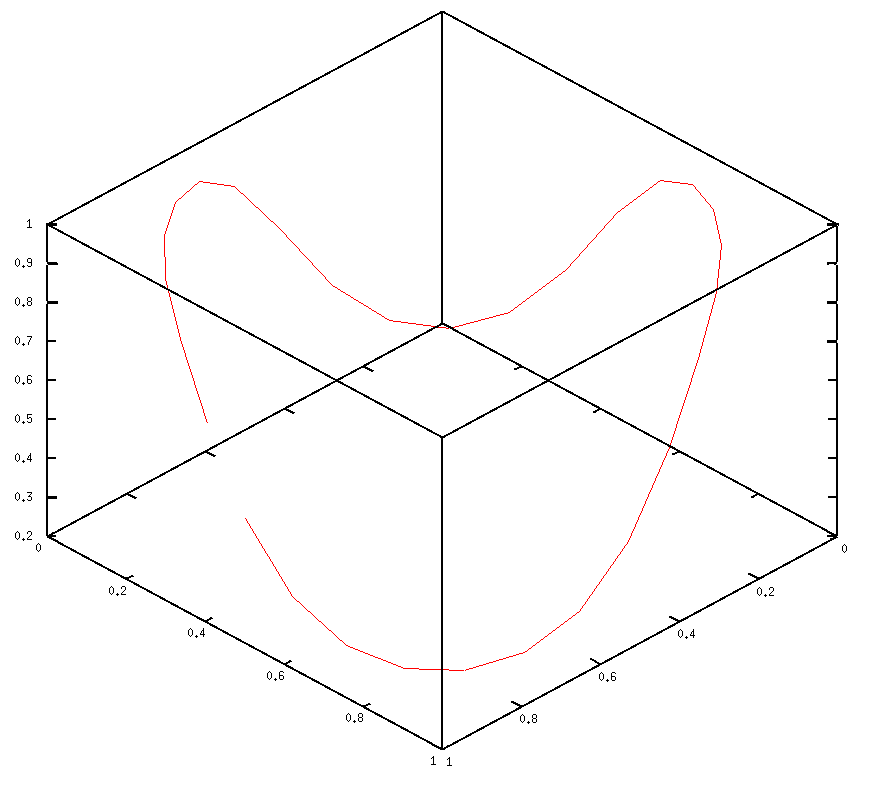
\includegraphics[scale=0.5]{img/xor1}
	\end{center}
	\caption{XOR function}
	\label{fig:xor1}
\end{figure}

\begin{figure}[tb]
	\begin{center}
		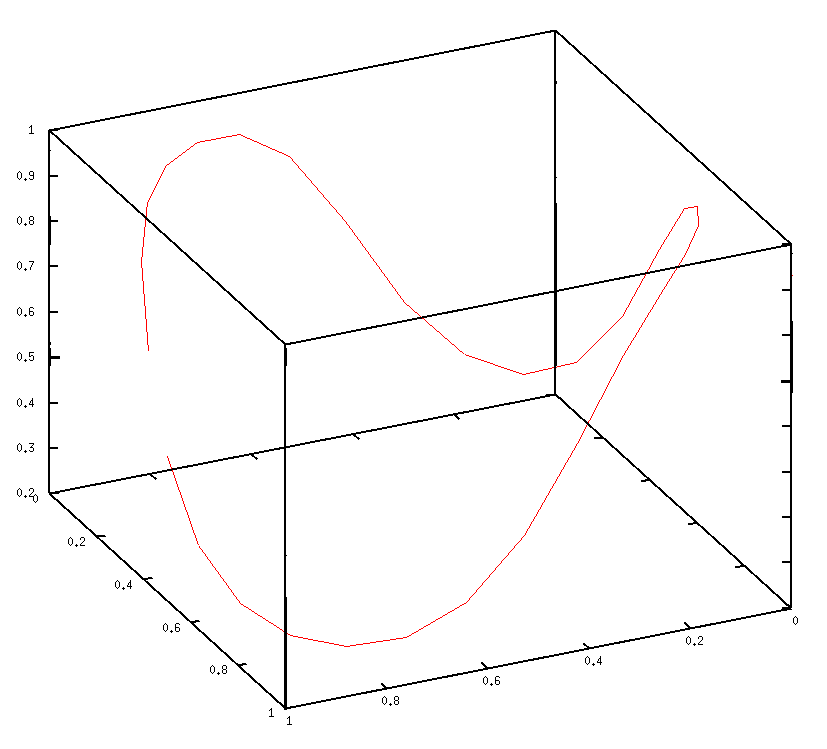
\includegraphics[scale=0.5]{img/xor2}
	\end{center}
	\caption{XOR Function}
	\label{fig:xor2}
\end{figure}

\begin{figure}[tb]
	\begin{center}
		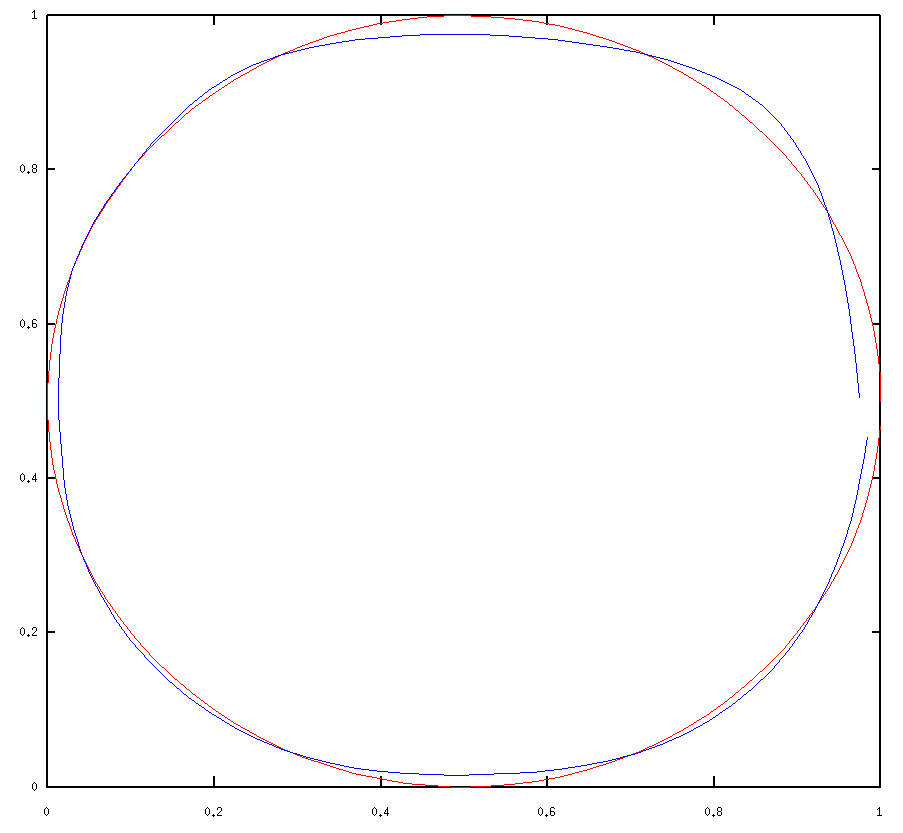
\includegraphics[scale=0.5]{img/circle}
	\end{center}
	\caption{Parametric Circle Function}
	\label{fig:circle}
\end{figure}

\begin{figure}[tb]
	\begin{center}
		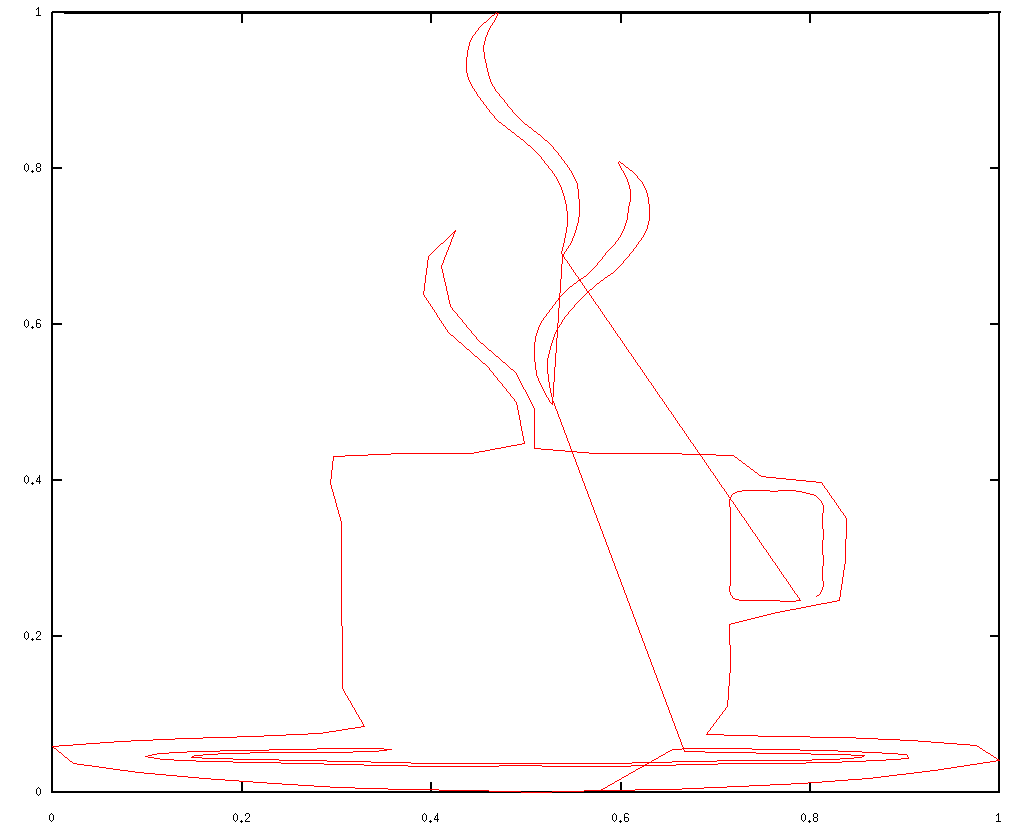
\includegraphics[scale=0.45]{img/coffee1}
	\end{center}
	\caption{Parametric Coffee Function}
	\label{fig:coffee1}
\end{figure}

\begin{figure}[tb]
	\begin{center}
		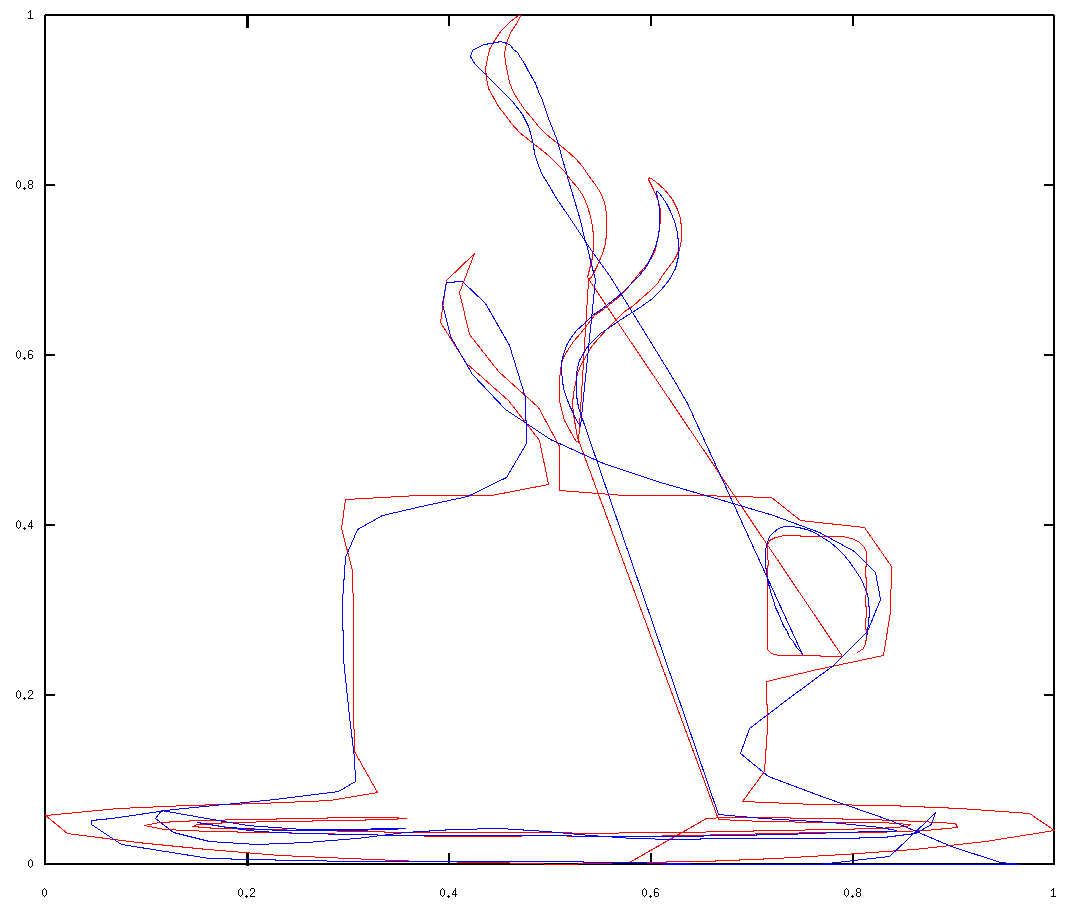
\includegraphics[scale=0.4]{img/coffee4}
	\end{center}
	\caption{neural Coffee Approximation in Blue}
	\label{fig:coffee4}
\end{figure}

\begin{figure}[tb]
	\begin{center}
		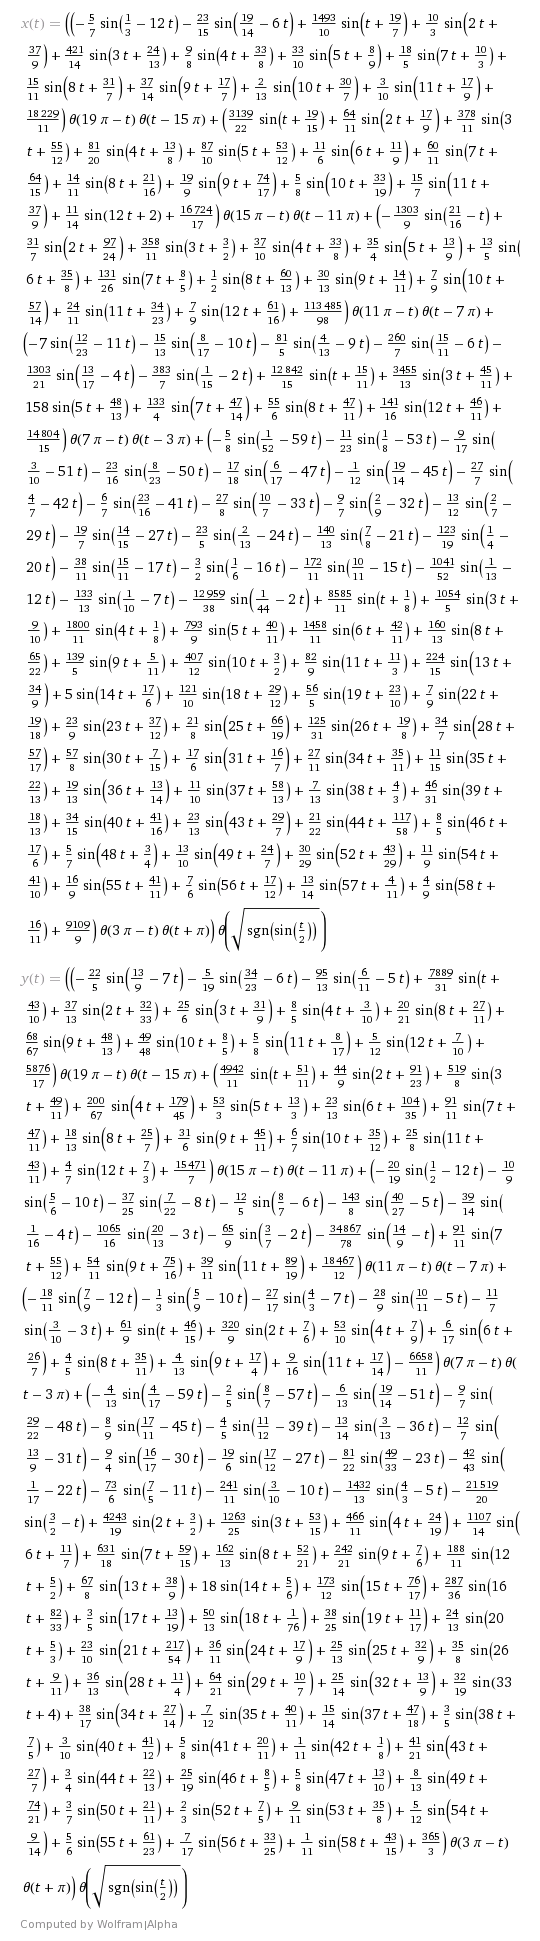
\includegraphics[height=0.9\textheight]{img/coffee-cup-eqns}
	\end{center}
	\caption{Equations for Coffee Cup}
	\label{fig:coffee-eqns}
\end{figure}

%\begin{table}[ht]
	%\caption{Sample Weather Predictions}
	%\begin{tabular}[cccccc]
		%& MIN & MAX & DEP & WNDSPD & WNDDR \\
	%\end{tabular}
	%\label{tab:weather}
%\end{table}

%\vspace{3in}
%\section{Coffee Cup Equation}
%\nopagebreak
%\begin{center}
%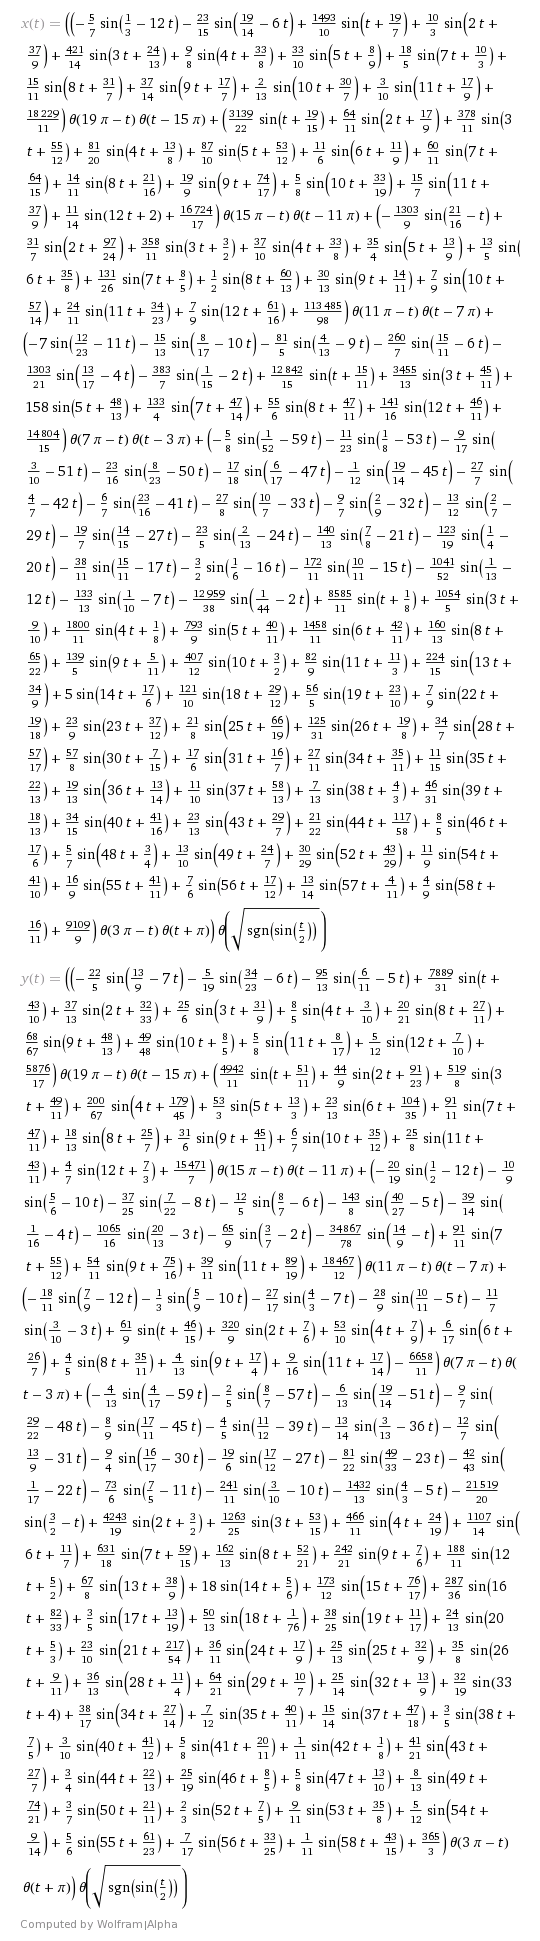
\includegraphics[height=\textheight]{img/coffee-cup-eqns}
%\end{center}

\end{document}

% citations:
% weather data
